\begin{figure*}[t]
\centering
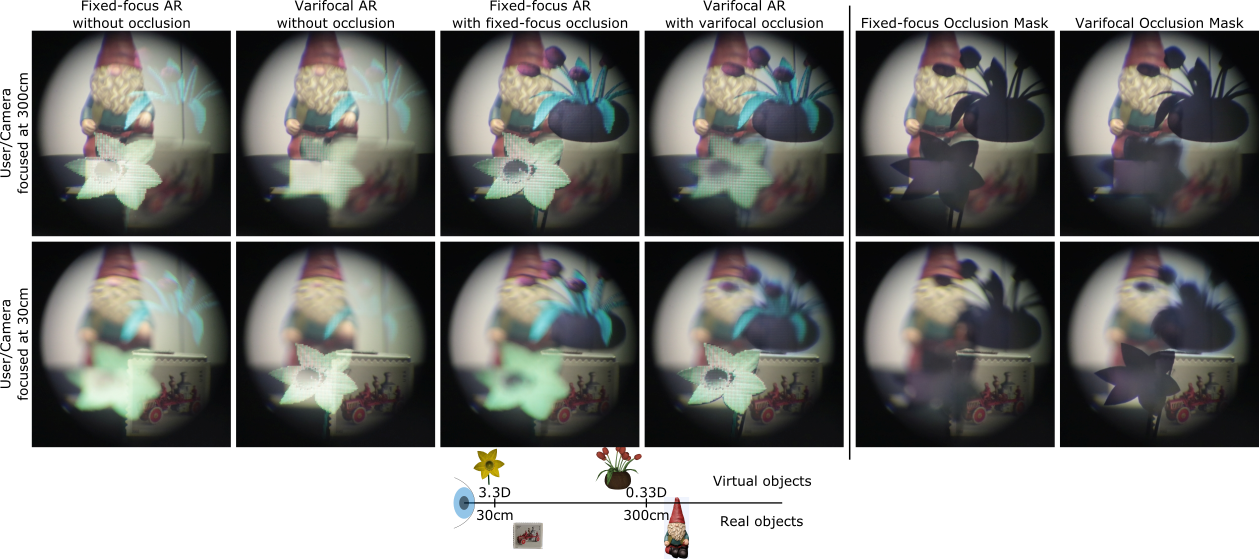
\includegraphics[width=0.99\textwidth]{images/varifocal_occlusion/teaser}
%\fbox{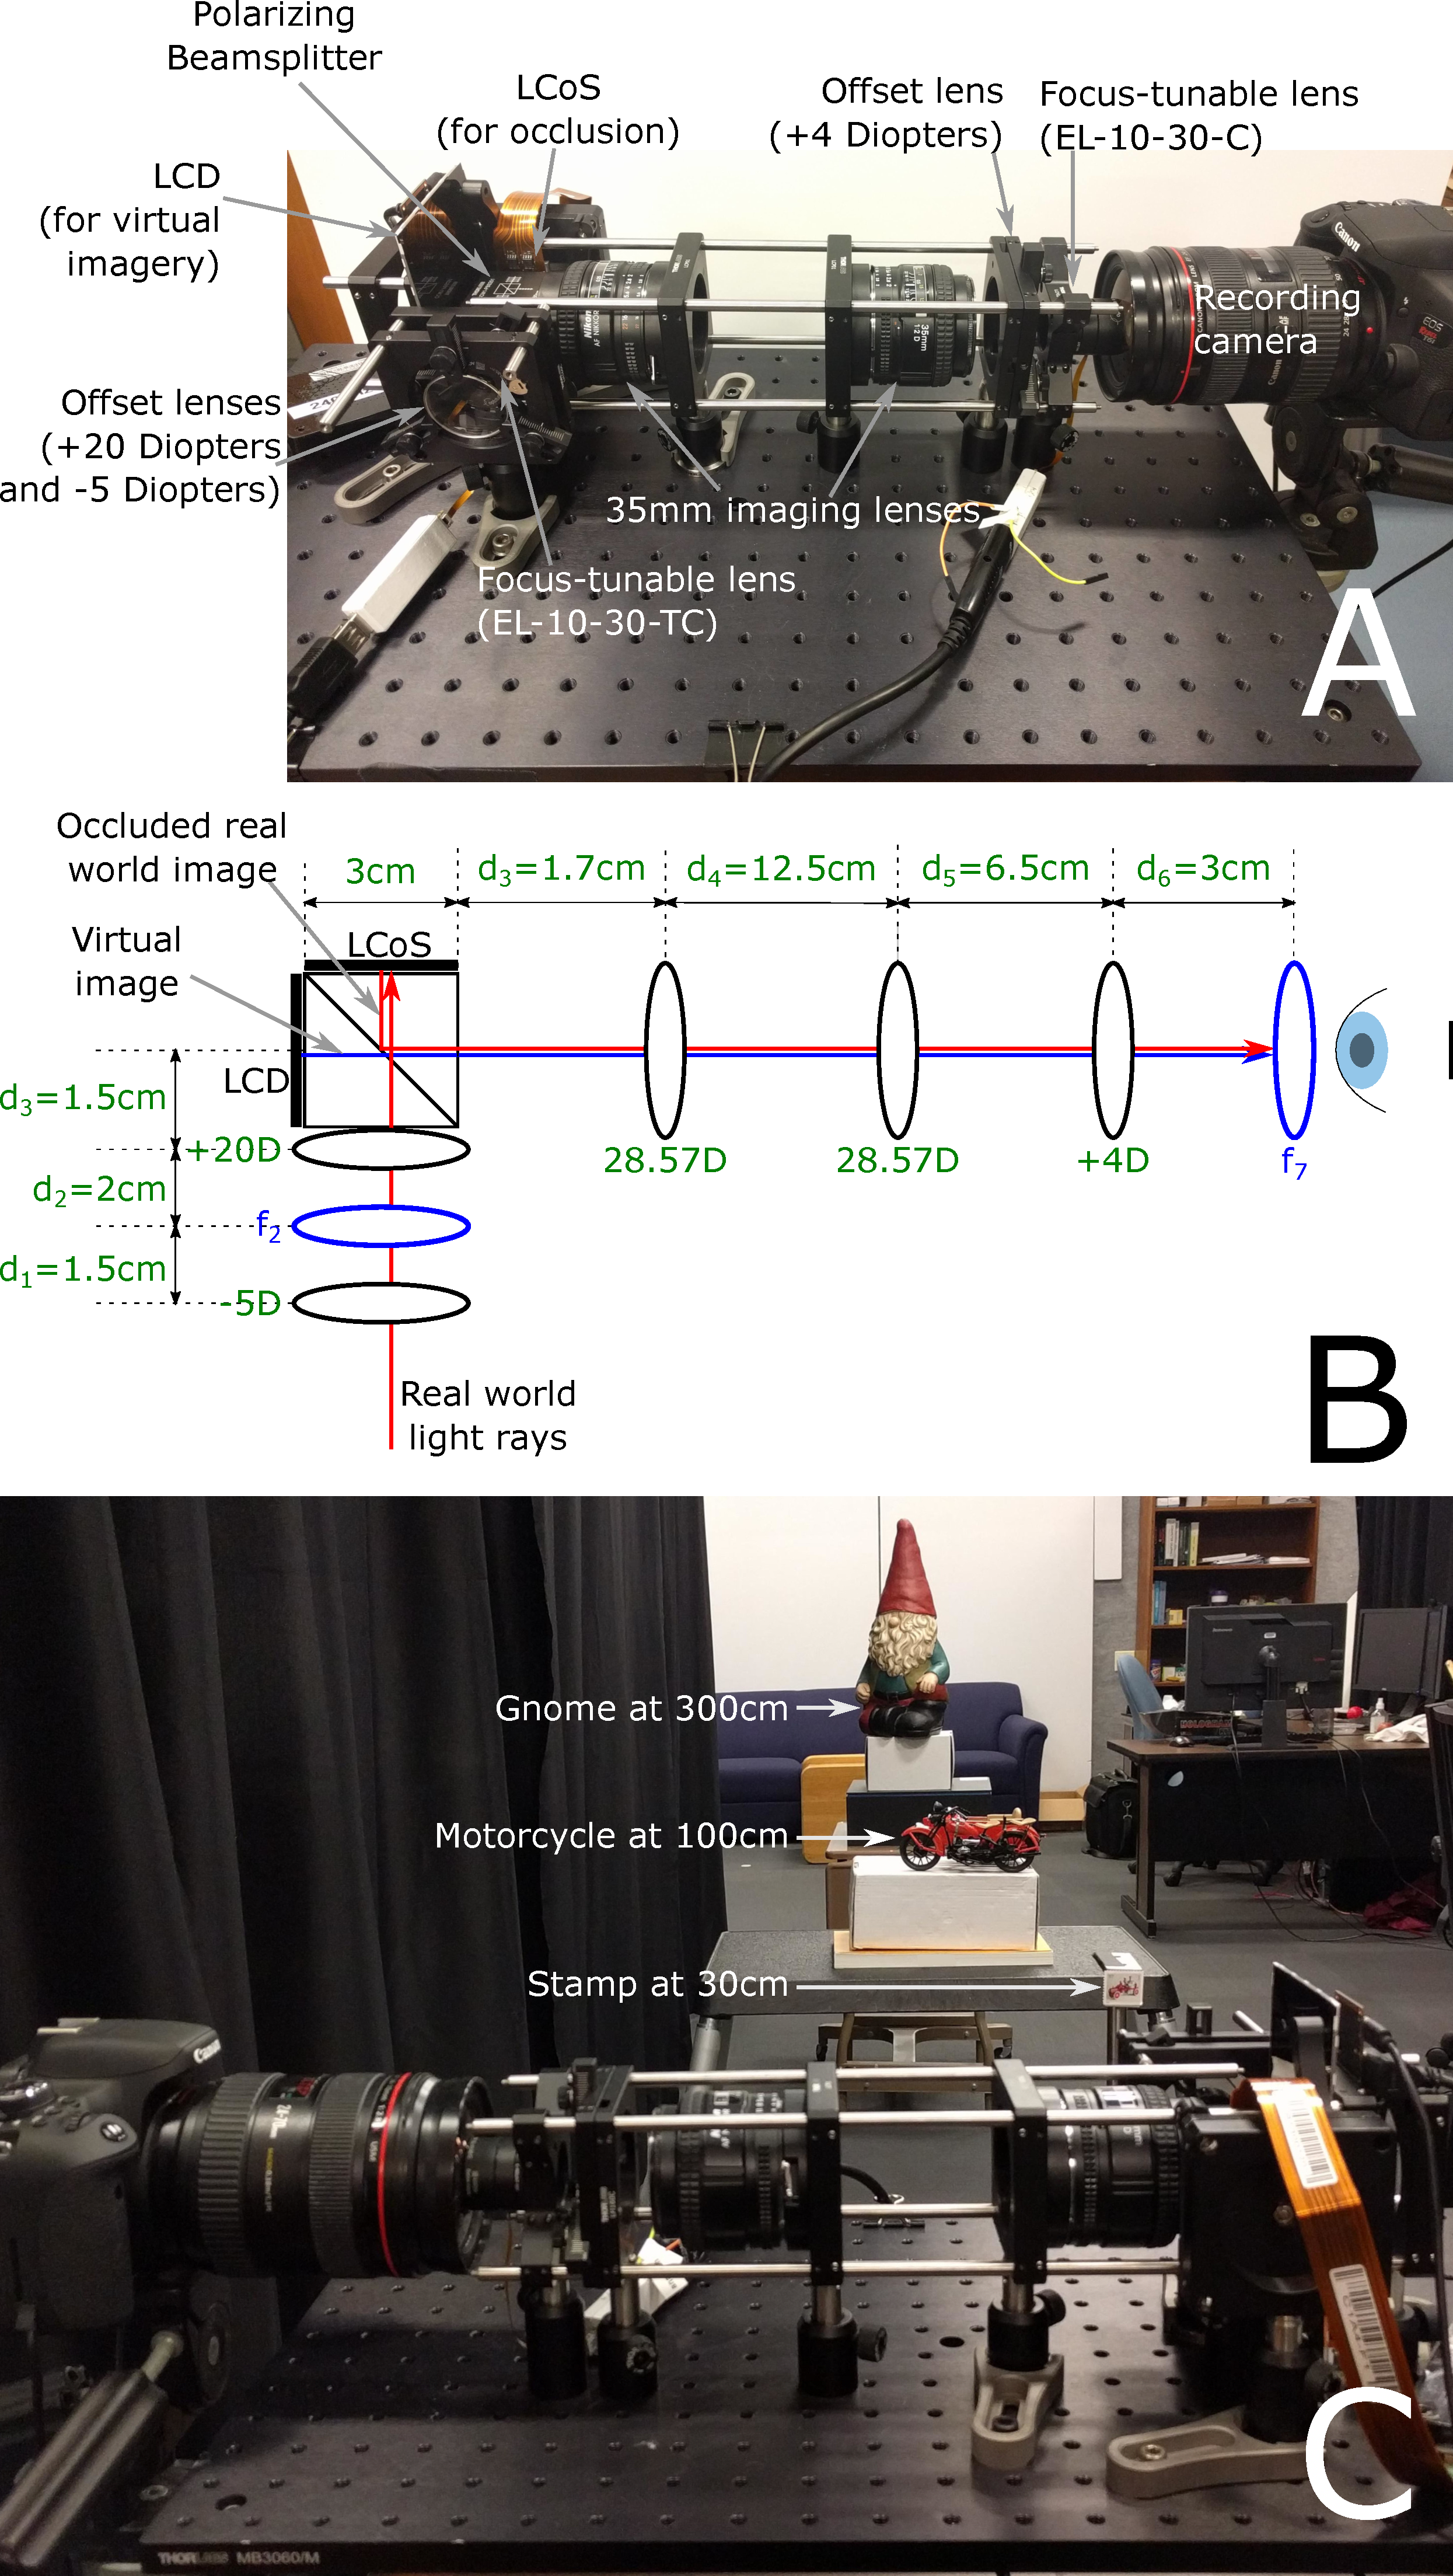
\includegraphics[width=0.46\textwidth]{images/prototype}}
\caption[Varifocal-Occlusion NED: teaser]{\textbf{Left of the vertical line:} views through our prototype AR display, which is emulating different AR display technologies for each column. 
The augmented scene is composed of real-world objects (stamp, motorcycle, and gnome) and virtual objects (ring, teapot, and bull). Objects are distributed at different depths: stamp and ring at 30cm, motorcycle and teapot at 100cm, and gnome and bull at 300cm. 
\textit{(Column 1)} Commercially available AR displays: a transparent virtual image is presented at a fixed distance. Important depth cues such as occlusion and accommodation are absent.
\textit{(Column 2)} Varifocal AR displays: virtual image can be moved to different depths, but images are still transparent. 
\textit{(Column 3)} Fixed-focus occlusion-capable AR display: 
Occlusion and virtual image is fixed at a single depth, limiting realism when the user is focused to other depths. Note how all virtual objects, including the nearby ones, are in focus when the camera is focused far, and all virtual objects are defocused when the camera is focused near. 
\textit{(Column 4)} Varifocal occlusion-capable AR displays: virtual and occlusion image plane can be moved to different depths enabling perceptually correct depth cues for occlusion and accommodation. Note how objects at the same depth, e.g., near objects (stamp and ring) or far objects (gnome and bull), are correctly in focus or defocused depending on the focus state of the user/camera.
\textbf{Right of the vertical line:} Comparison of occlusion masks between fixed-focus and varifocal occlusion-capable displays.}
\label{fig:varifocal_occlusion:teaser}
\end{figure*}


Augmented Reality (AR) systems offer unprecedented experiences and are considered a next-generation computing platform. These wearable displays promise to seamlessly augment the physical world around us with digital content, such as information displays or user interfaces. Providing a seamless, perceptually realistic experience, however, requires the display to accurately support all depth cues of the human visual system~\cite{Palmer:1999,Howard:2002}. While current AR displays offer impressive capabilities, they typically do not support the most important depth cue: occlusion~\cite{cutting1995perceiving}.

Providing accurate, i.e., mutually consistent and hard-edge, occlusion between digital and physical objects with optical see-through AR displays is a major challenge. When digital content is located in front of physical objects, the former usually appear semi-transparent and unrealistic (see Fig.~\ref{fig:varifocal_occlusion:teaser}, columns~1 and~2). To adequately render these objects, the light reflected off of the physical object toward the user has to be blocked by the display before impinging on their retina. This occlusion mechanism needs to be programmable to support dynamic scenes and it needs to be perceptually realistic to be effective. The latter implies that occlusion layers are correctly rendered at the distances of the physical objects (see Fig.~\ref{fig:varifocal_occlusion:depth-dependent-occlusion}), allowing for pixel-precise, or hard-edge, control of the transmitted light rays.

Recent proposals on occlusion-capable optical see-through (OST) displays have only partially addressed this challenge. Global dimming~\cite{Mori2018}, for example, is successful in controlling the light transmission of the display but without spatial control. Image-forming systems~\cite{Kiyokawa2003,Cakmakci2004,Gao2012} enable consistent occlusions, but these are only correct at a single distance, severely limiting the image quality at other depths (see Fig.~\ref{fig:varifocal_occlusion:teaser}, column~3) and requiring bulky relay optics. Spatial light modulators (SLMs) for occlusion control can also be used without relay optics~\cite{Itoh2017}, but these will always be out of focus and require additional compensation techniques. Light field-based occlusion technology~\cite{maimone2013general} offers somewhat sharper occlusion control without relay optics. Out-of-focus SLMs~\cite{maimone2013general,Itoh2017} are usually based on liquid crystal displays (LCDs), which introduce diffraction artifacts of the physical world observed in OST displays, thus limiting the perceived image quality.

With this work, we introduce varifocal occlusion-capable optical see-through AR displays. These systems aim at providing a seamless and perceptually realistic experience by providing mutually consistent occlusions over a large depth range (see Fig.~\ref{fig:varifocal_occlusion:teaser}, column~4). Similar to varifocal near-eye displays, our approach uses focus-tunable lenses to dynamically shift the occlusion SLM to a single, but adaptive, optical distance. We envision this approach to operate in a gaze-contingent mode, where an eye tracker determines the distance of the fixated object and both the digital content and the occlusion system are dynamically focused at this distance. 

A unique challenge of varifocal occlusion implemented with focus-tunable optics is precise control of the optical distortion of the physical light. As lenses change their focal power to align the occlusion SLM with different distance of the physical scene, the latter may also be magnified and its perceived distance altered, because the light of the physical scene and the occlusion SLM must share the same optical path. We derive a formal optimization approach and real-time heuristics to drive the proposed system in a perceptually accurate manner, preventing optical distortions of the physical world. 

Specifically, we make the following contributions:
%
\begin{enumerate}
\item We introduce varifocal occlusion as an AR display capability that adaptively changes the focal distance of an occlusion mask to enable hard-edge occlusion over a large depth range. 
\item  We develop an optimization-based optical design approach for our focus-tunable optical system to achieve varifocal occlusion in a perceptually realistic manner without optically distorting the observed scene. 
\item Using insights gained from the optimization approach, we use a ray-transfer matrix approach to derive closed-form solutions for optical designs that allow for varifocal occlusion in real-time.
\item We implement a monocular varifocal occlusion-capable AR display and demonstrate improved realism through depth-dependent occlusion.
\end{enumerate}

\begin{figure}[t]
\centering
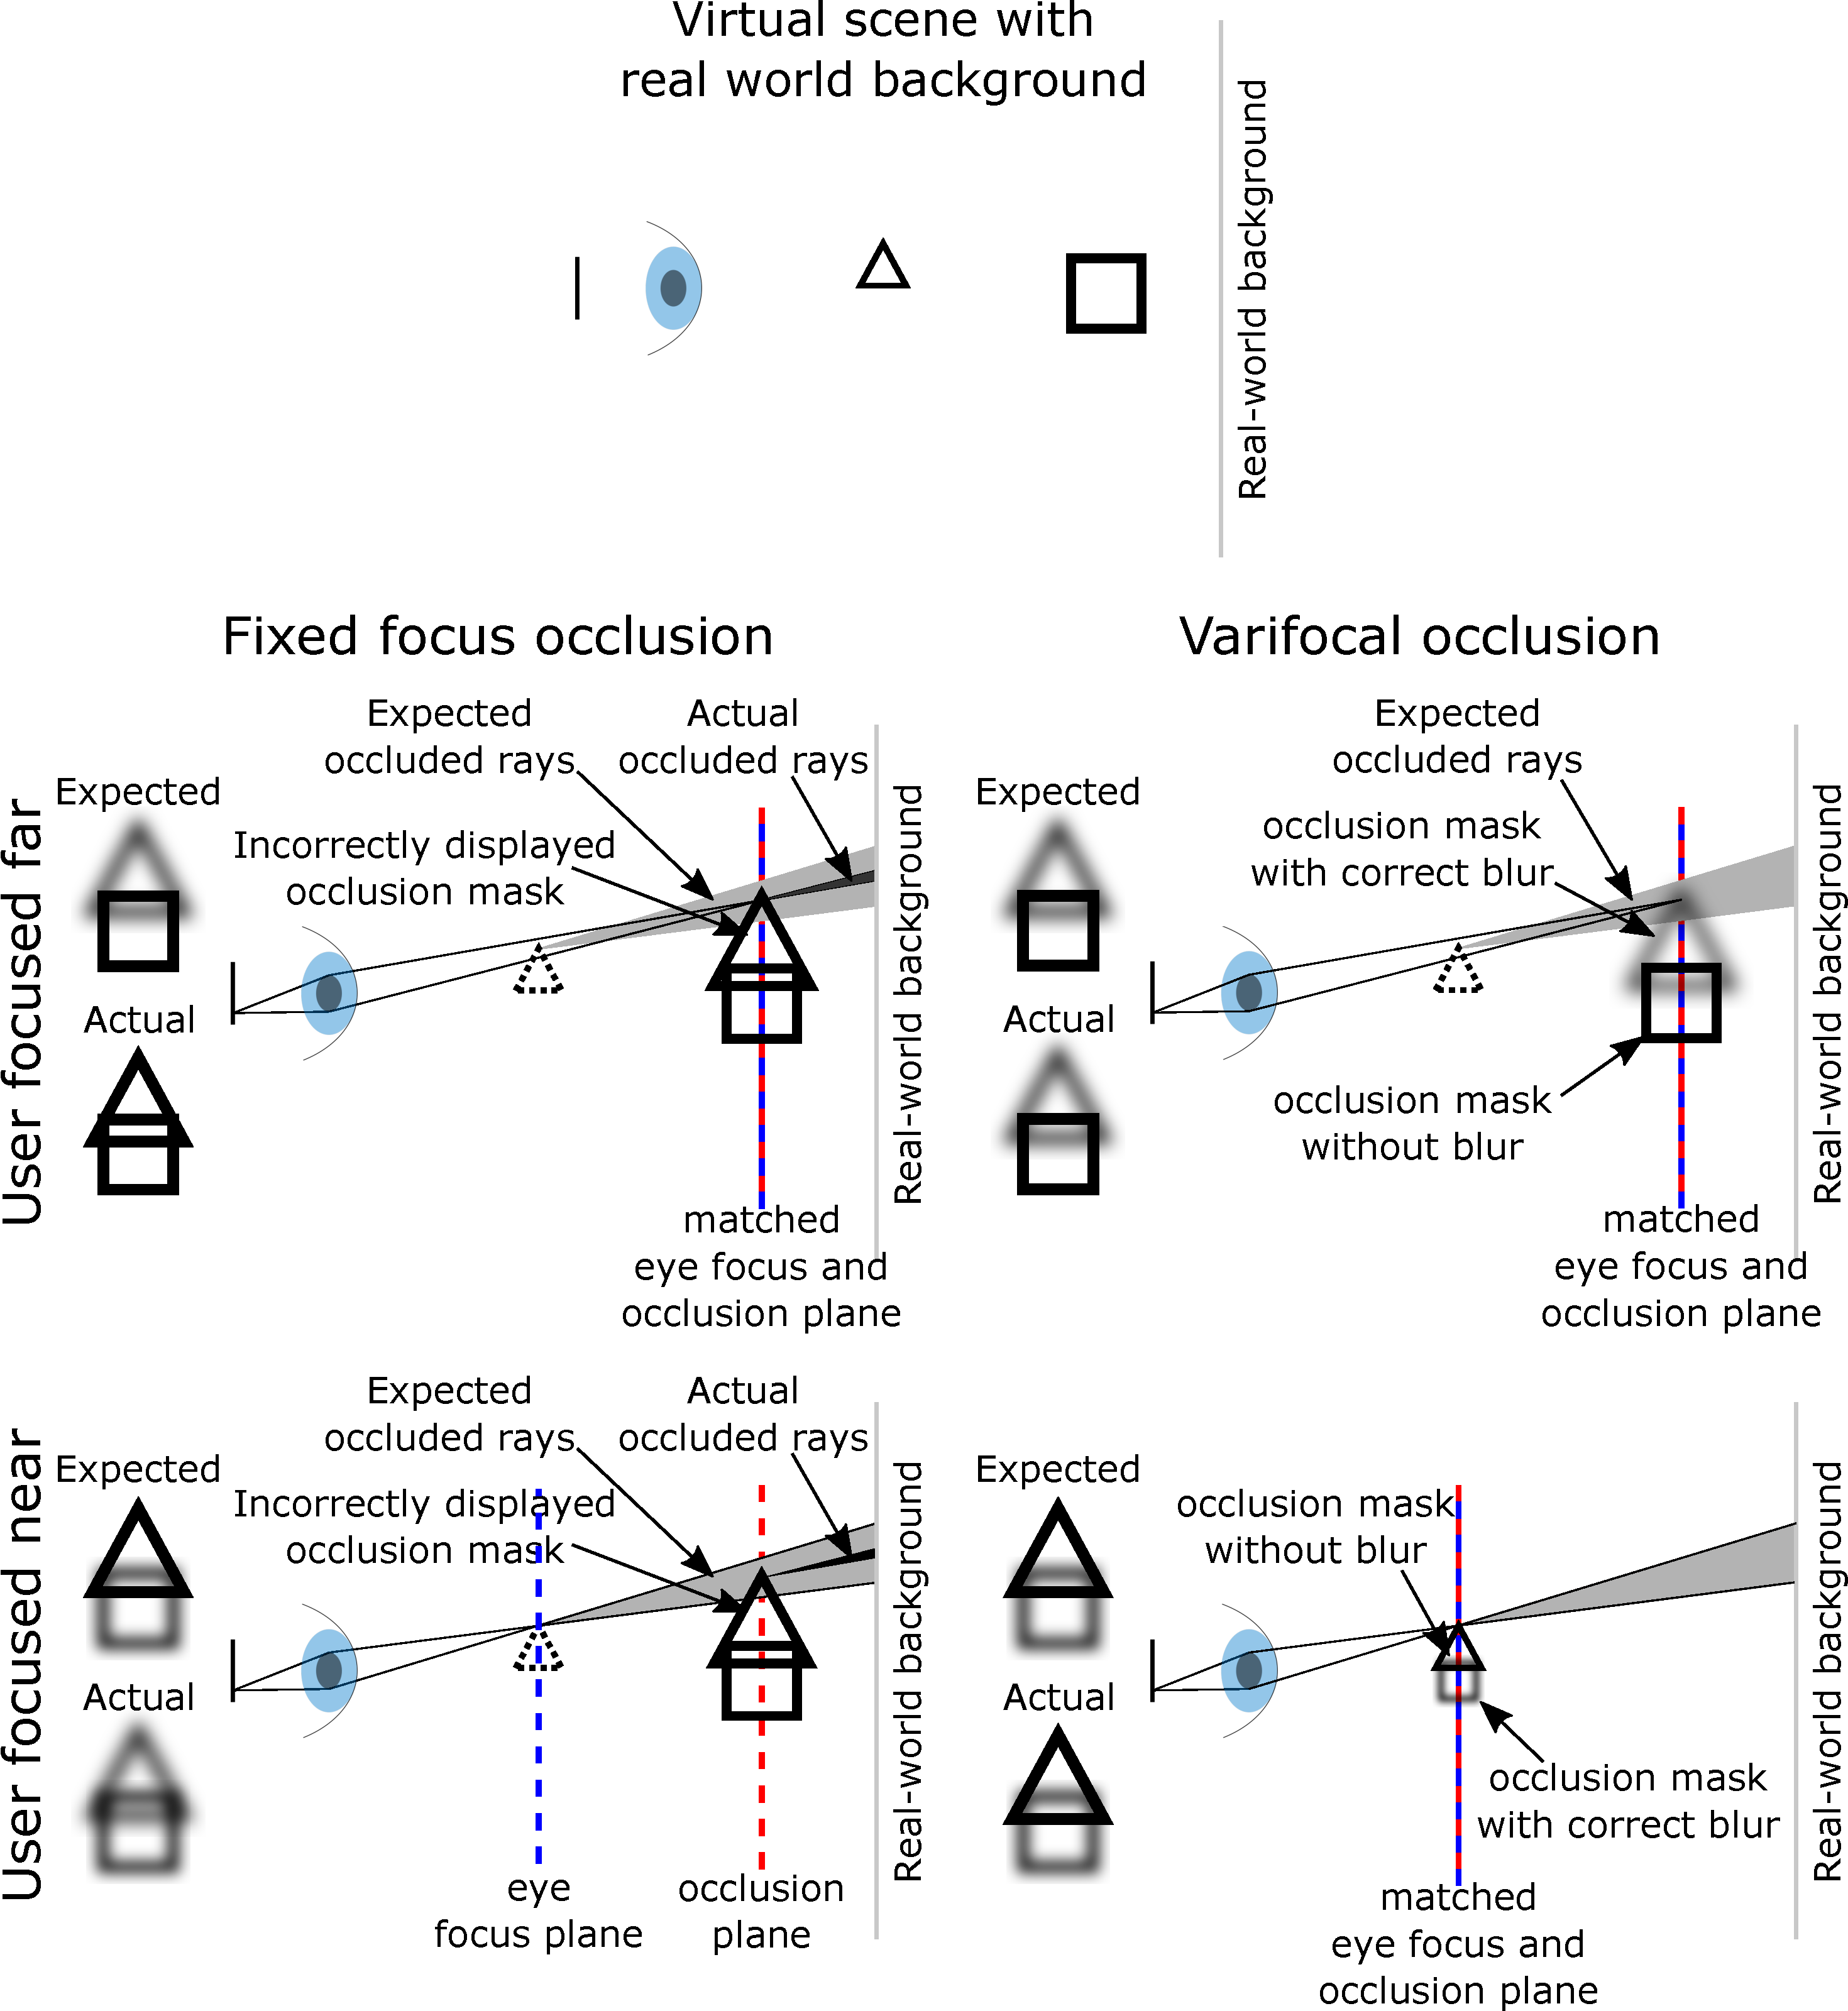
\includegraphics[width=0.9\columnwidth]{images/varifocal_occlusion/depth-dependent-occlusion}
%\fbox{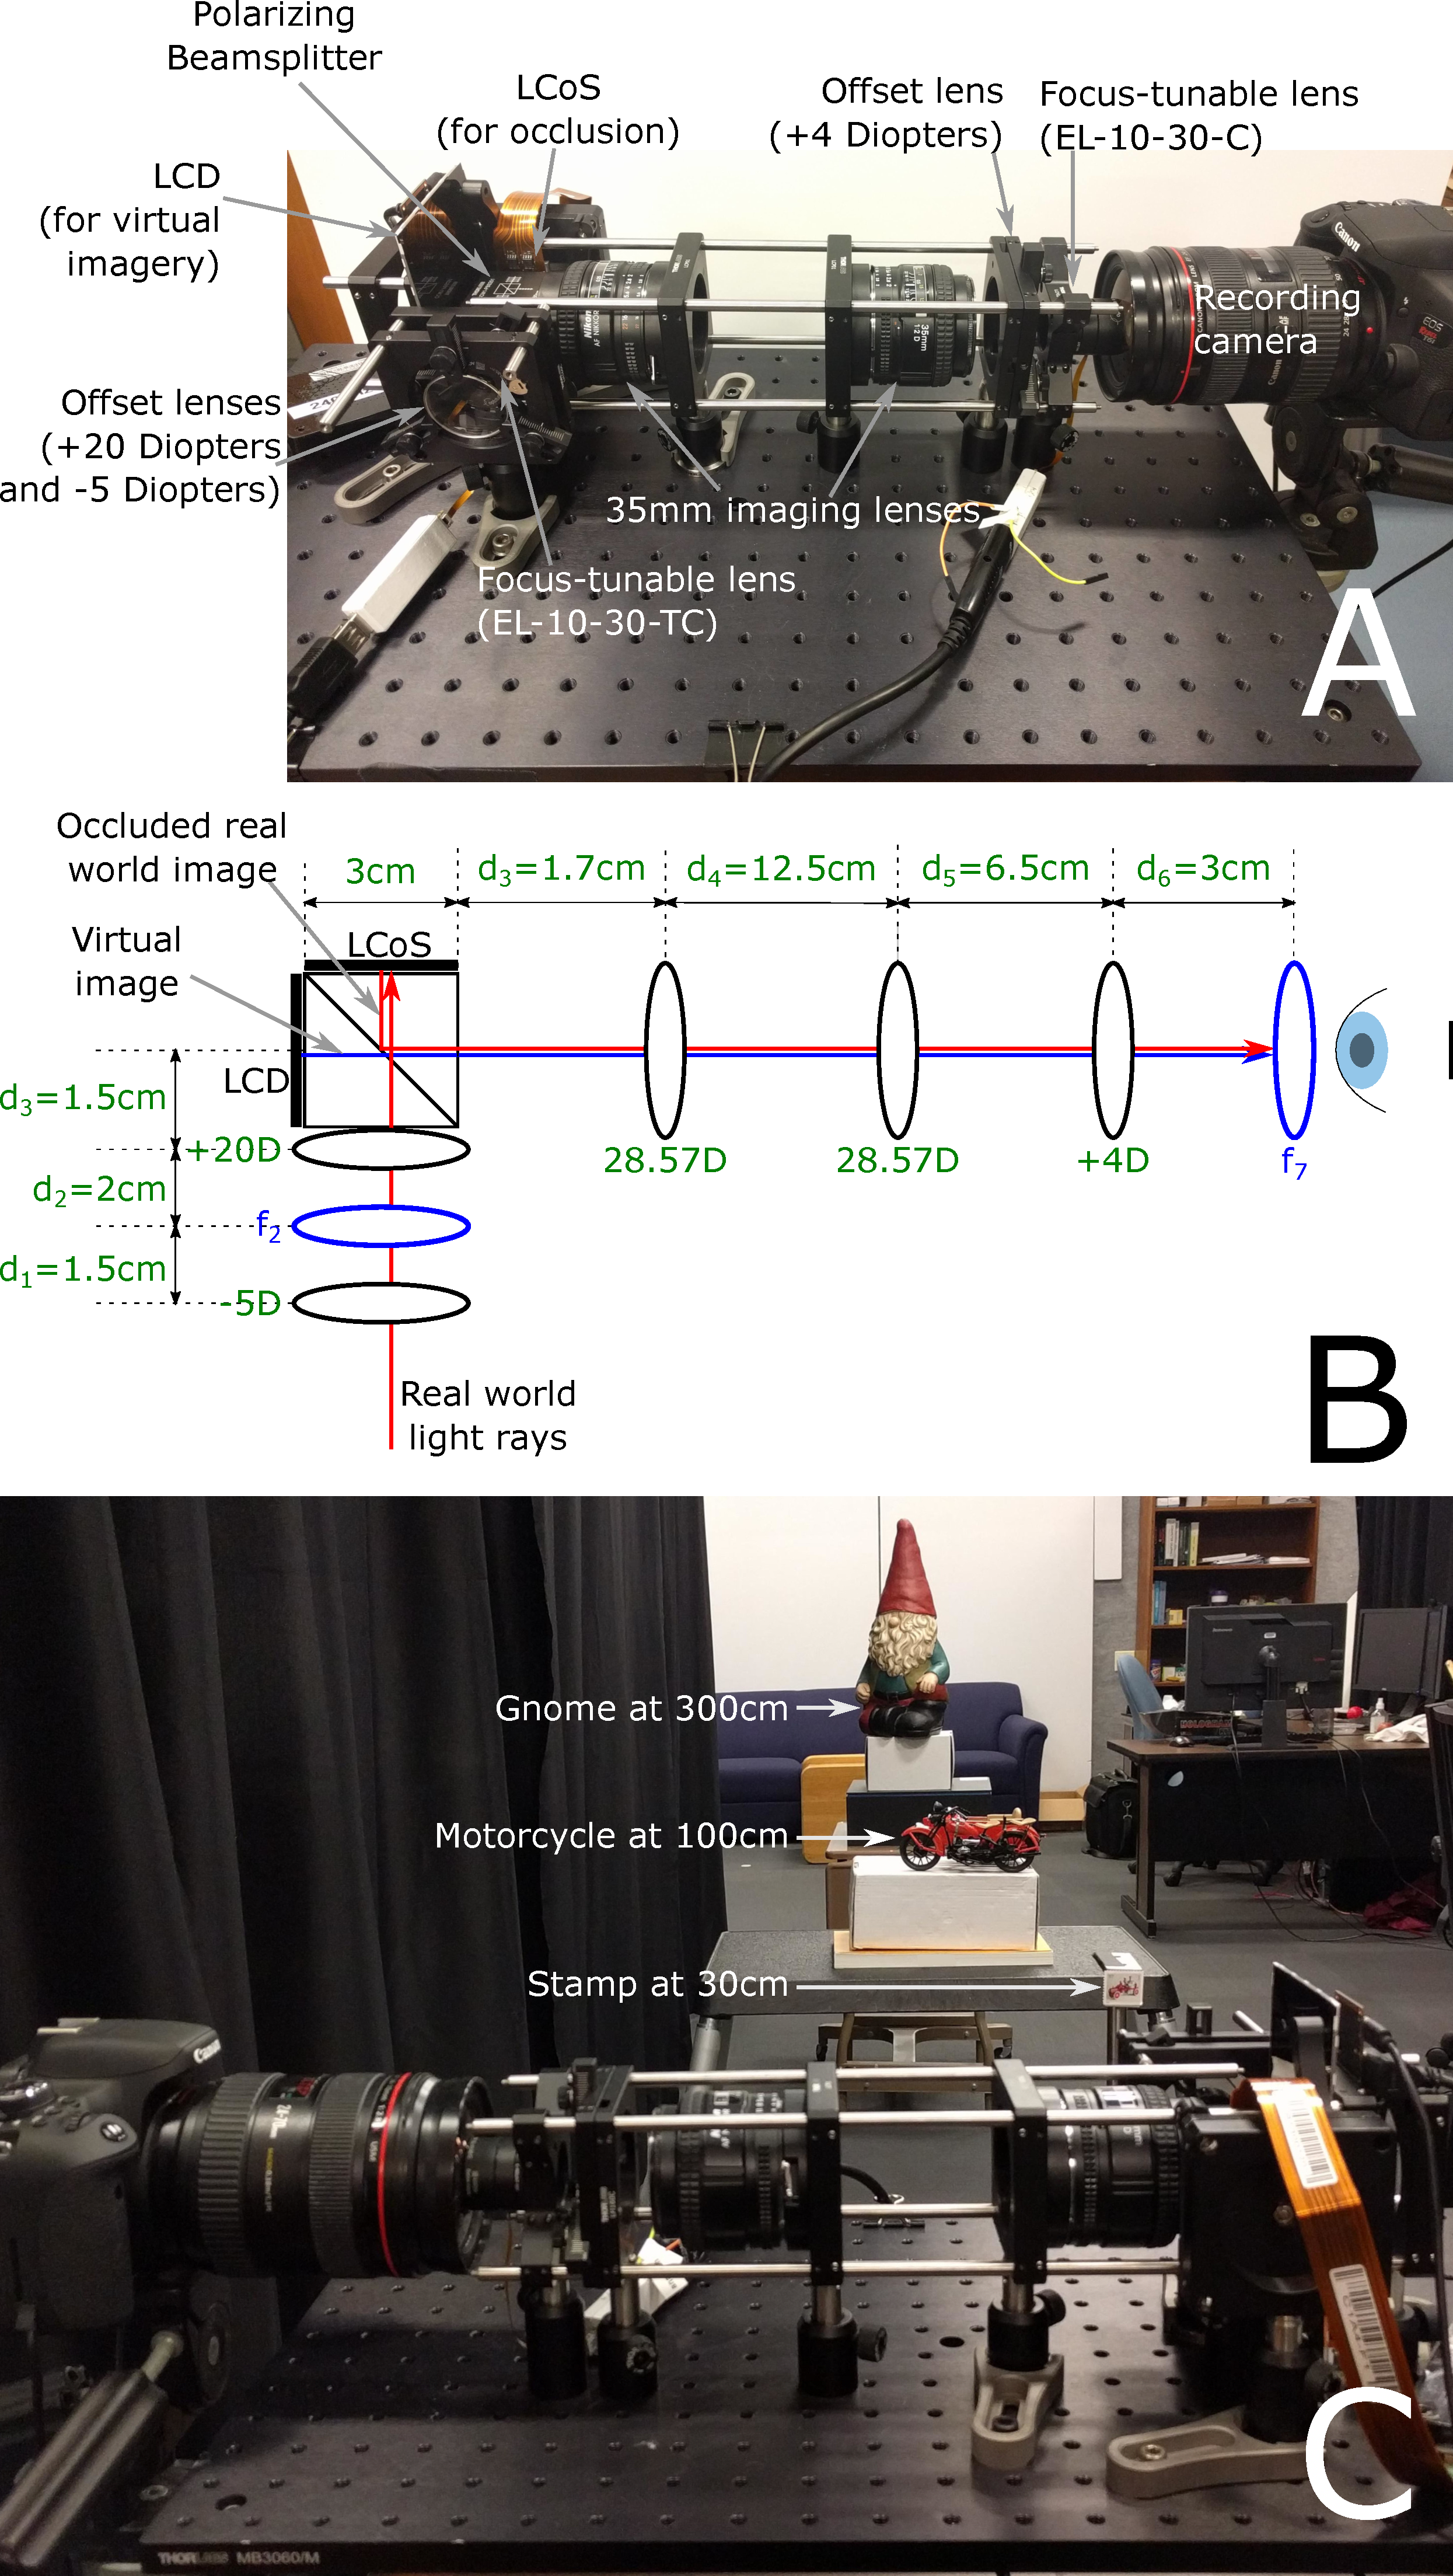
\includegraphics[width=0.46\textwidth]{images/prototype}}
\caption[Varifocal-Occlusion NED: concept of depth-dependent occlusion]{\emph{Topmost Row:} A virtual scene composed of one near and one far object placed in front of a real-world background. \emph{Grid of figures:} Comparison of occlusion mechanism only (i.e. ignoring the digital or color image) for fixed-focus and varifocal occlusion displays for the above scene. Dashed blue and red lines indicate the user's focal plane and display's occlusion image plane respectively. Solid black lines indicate image formation for content placed in the user's focal plane. Images next to the eye show the ``Expected" and ``Actual" images seen by the user. Note that for fixed-focus occlusion, the occlusion plane is always at the far distance which causes the nearby object's occlusion mask to be seen incorrectly always and the far object's occlusion mask to be seen incorrectly when the eye is focused nearby. Varifocal occlusion-capable displays, on the other hand, move the occlusion plane to the user's focal plane and display an occlusion mask for in-focus objects as it is and a perceptually correct occlusion mask for out-of-focus objects by applying a computational blur.}
\label{fig:varifocal_occlusion:depth-dependent-occlusion}
\end{figure}


